% !TeX encoding=unicode
% !TeX spellcheck = de-DE

\chapter{Theoretical foundations}
%
\section{Basics of perturbative QCD}
QCD is the quantum field theory that describes the strong interactions between Quarks and Gluons.
Mathematically, it is a non-abelian gauge theory with symmetry group SU(3).
Its Lagrangian is given by
%
\begin{equation}
  \Lagr_\text{QCD} = \sum_q \bar\psi_{q,a} (i \gamma^\mu \partial_\mu \delta_{ab} - g_s \gamma^\mu t_{ab}^C \glufield_\mu^C - m_q \delta_{ab}) \psi_{q,b} - \frac{1}{4} F_{\mu \nu}^A F^{A \, \mu \nu} \, ,
\end{equation}
%
where the sum goes over all quark flavors.
The $\psi_{q,a}$ are quark-field spinors, where $a=1 \dots 3$ denotes the color index, and the $\glufield_\mu^C$ are gluon fields with a color index $C=1 \dots 8$.
The strong coupling constant is denoted by $g_s$.
Quarks transform under the fundamental representation of SU(3) while gluons transform under the adjoint representation.
The $t_{ab}^C$ are  the generators of the group.
The gluon field tensor $F_{\mu \nu}^A$ is given by
%
\begin{equation}
	F_{\mu \nu}^A = \partial_\mu \glufield_\nu^A - \partial_\nu \glufield_\mu^A - g_s f_{ABC} \glufield_\mu^B \glufield_\nu^C \, ,
\end{equation}
%
where the $f_{ABC}$ are the structure constants of the group, defined through $[ t^A,t^B ] = i f_{ABC} t^C$.
In comparison to quantum electrodynamics (QED), the main difference is the presence of the interaction term $- g_s f_{ABC} \glufield_\mu^B \glufield_\nu^C$ which results in the existence of 3-gluon and 4-gluon vertices.

The perturbative approach to QCD is to write the observables as a power series in $\alpha_s = g_s^2/(4 \pi)$:
%
\begin{equation}
  F = F^{(1)} \alpha_s + F^{(2)} \alpha_s^2 + \dots \, ,
\end{equation}
%
where $\alpha_s \ll 1$ so that the series can be truncated after a few terms to obtain a useful approximation.
A straightforward way to determine the coefficients is the use of Feynman Diagrams.
%
\subsection{Renormalization and the running coupling}
Calculations in perturbative QCD involve UV-divergent diagrams such as the one illustrated in \cref{fig:loop}, which gives a contribution to the gluon self-energy.
Luckily QCD is a renormalizable theory and therefore the divergences can be handled by regularization and renormalization.
As a consequence, the quantities appearing in the Lagrangian (the \enquote{bare} quantities) are not the same as the quantities we observe physically.
The measured values depend on the energy scale, called \textit {renormalization scale} $\mu_R$, at which they are evaluated.
This scale is arbitrary and unphysical and if we consider the whole perturbative series, the scale dependence vanishes.
The scale dependence can be described by differential equations known as \textit{renormalization group equations}.
For example, the equation for the coupling constant takes the form
%
\begin{equation}
  \dod{ \alpha_{s} ( \mu_R^{2} ) }{ \ln{\mu_R^2} } = \beta(\alpha_s(\mu_R^2)) = - \alpha_s^2 (b_0 + b_1 \alpha_s + b_2 \alpha_s^2 + \dots) \, .
	\label{eq:rge}
\end{equation}
%
The minus sign in \cref{eq:rge} is responsible for the asymptotic freedom of QCD:
As the momentum transfer becomes large, the strong coupling becomes weak so that quarks and gluons nearly behave as if they were free particles.
%
\begin{figure}[]
	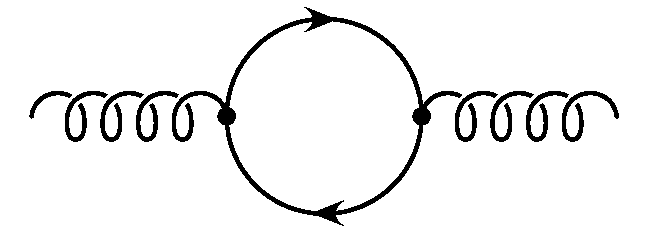
\includegraphics[width=0.3\textwidth]{images/loop.pdf}
	\caption{UV-divergent loop diagram}
	\label{fig:loop}
\end{figure}
%

In leading order the analytic solution for \cref{eq:rge} is known as \textit{running couplig} and given by
%
\begin{equation}
	\alpha_s(\mu_R^2) = \frac{\alpha_s(\mu_0^2)}{1 + b_0 \alpha_s(\mu_0^2) \ln \frac{\mu_R^2}{\mu_0^2}} = \frac{1}{b_0 \ln \frac{\mu_R^2}{\Lambda^2}} \quad \text{with} \quad b_0=\frac{11 N_C - 2 n_f}{12 \pi} \, ,
\end{equation}
%
where $N_C$ is the number of colors and $n_f$ denotes the number of flavors.
Note that this is only valid at scales where $n_f$ does not change.
The first expression uses a reference scale $\mu_0$, where the value of $\alpha_s$ is known whereas the second one uses the constant $\Lambda$, which is the scale where the coupling would diverge.
%
\section{The Parton Model}
The parton model was introduced in 1969 by Richard P. Feynman to describe high-energy particle collisions involving hadrons \cite{feynman1969}.
The basic assumption of the parton model is that all hadrons consist of point-like particles (partons) which are responsible for their behavior in interactions.
In QCD these can be identified as quarks and gluons.
Furthermore, it is assumed that the hadron is in a reference frame where it carries infinite (or at least very high) momentum.
In this infinite momentum frame the hadron suffers both Lorentz contraction and time dilation so that the distribution of partons within it does not change during the (vanishingly small) time of interaction.
Thus each parton carries a definite fractional momentum $x$, with $0<x<1$.
In addition, the process of hadronization due to quark confinement happens too late to influence the interaction.
Another important consequence is that the probability of a parton influencing the scattering of another parton is suppressed (\enquote{incoherence} of the parton model).
The reason this model works is the asymptotic freedom of the underlying theory.
However, this also limits the applicability of the parton model to high energy cross sections.

With the help of perturbative QCD, there is a class of reactions involving hadrons for which the cross sections can be calculated directly.
These reactions are inclusive and do not contain any hadrons in the initial state.
A simple example is lepton pair annihilation into hadrons.
As the hadronic final state is fully inclusive, the cross section is identical to the electroweak cross section for $l+l' \rightarrow q \bar q$, where $l$ and $l'$ denote leptons and $q$ ($\bar q$) denotes a (anti-)quark.
Assuming $e^+ e^-$ annihilation and energies much less than the Z boson mass, the total cross section is therefore given by
%
\begin{equation}
  \sigma_{e^+ e^- \rightarrow q \bar q}(s) = \frac{4 \pi \alpha^2}{3 s} \cdot 3 \sum_f Q_f^2 \, ,
	\label{eq:e+e-_annihilation}
\end{equation}
%
where the sum is over all quark flavors that can be produced at the center-of-mass energy $\sqrt s$ and the factor $3$ is the number of colors \cite{cteq2001}.
%
%\subsection{Lepton-Hadron Cross Sections}
%In the parton model, cross sections involving hadrons in the initial state are calculated by combining the parton-level cross sections (in leading order) with probability densities for a specific parton to be involved in it.
%For example, the total cross section for scattering of a hadron by a lepton (\figref{fig:dis}) can be written as
%%
%\begin{equation}
%	\sigma^{(lh)} (x,Q^2) = \sum_f \int_x^1 \dif \xi \enspace \hat \sigma^{(lf)} (x / \xi, Q^2) \cdot \phi_{f/h}(\xi) \, .
%\end{equation}
%%
%\begin{figure}[]
%	\includegraphics[width=0.5\textwidth]{images/dis.pdf}
%	\caption{Deeply inelastic scattering.}
%	\label{fig:dis}
%\end{figure}
%%
%where $\phi_{f/h}(\xi)$ is the probability density for finding a parton of flavor $f$ with fractional momentum $\xi$ in hadron $h$.
%This is generally called a \textit{parton distribution function} (PDF).
%The variables $x$ and $Q^2$ are commonly used to describe this process, which is called \textit{deeply inelastic scattering}, and are defined as follows:
%%
%\begin{align}
%  	Q^2 &= -q^2 = -(k - k')^2		\quad \text{(momentum transfer)} \\
%	x &= \frac{Q^2}{2 p \cdot q}	\quad \text{(Bjorken scaling variable)}
%\end{align}
%%
%$k$ and $k'$ are the momenta of the lepton before and after the scattering while $p$ is the momentum of the initial hadron.
%The cross section for elastic scattering of the parton, $\hat \sigma^{(lf)}$, can be calculated in the Born approximation.
%
%In deeply inelastic scattering, the PDFs are related to structure functions $F_i(x,Q^2)$.
%These can experimentally be obtained by measuring the differential cross section, which (considering photon exchange only) is related to the structure functions by
%%
%\begin{equation}
%	\frac{\dif \sigma^{(lh)}}{\dif x \dif y} = 8 \pi \alpha^2 \frac{m_h E}{Q^4} \left[ \frac{y^2}{2} 2 x F_1(x,Q^2) + \left( 1 - y - \frac{m_h x y}{2 E} \right) F_2(x,Q^2) \right] \, ,
%\end{equation}
%%
%where $y = \frac{p \cdot q}{p \cdot k}$ describes the inelasticity.
%Therefore, deep inelastic scattering can be used to determine the PDFs.
%The structure functions have two interesting properties:
%%
%\begin{enumerate}[labelindent=\parindent,leftmargin=*]
%	\item in the \textit{Bjorken limit} $Q^2,\nu  \rightarrow \infty$ with $x$ fixed, the structure functions depend only on $x$, not on $Q^2$ (\textit{scaling});
%	\item the structure functions satisfy the \textit{Callan-Gross relation}: $2 x F_1 = F_2$.
%\end{enumerate}
%%
%The first one implies that partons are point-like particles.
%The second is evidence for the spin-$\frac{1}{2}$ nature of quarks \cite{ellis1996}.
%%
\subsection{Hadron-Hadron Cross Sections}
One of the achievements of the parton model is the prediction of cross sections for hadron-hadron collisions such as the \textit{Drell-Yan process} $h(p) +  h'(p') \rightarrow l(k) + l'(k') + X$.
That is possible because PDFs are universal between reactions, so they can be determined once and used to calculate different cross sections.
In general, the cross section for a hard scattering process involving two initial hadrons can be written as
%
\begin{equation}
	\sigma(p,p') = \sum_{i,j} \int \dif \xi \dif \xi' \enspace \phi_{i/h}(\xi) \cdot \sigma_{ij}(\xi p,\xi' p',\alpha_s(\mu^2)) \cdot \phi_{j/h'}(\xi') \, .
\end{equation}
%

%\Cref{fig:Z_y_LO} shows the cross section as a function of the Z boson rapidity in a Drell-Yan process at $\sqrt{s}=\SI{7}{\tera\electronvolt}$ calculated with the Sherpa event generator \cite{gleisberg2008ta,schonherr2008,gleisberg2008fv,schumann2007}.
%The plot has been generated using the Rivet analysis system \cite{rivet2010}.
%Different PDFs have been used (For each PDF set the central value has been used. The inherent uncertainties are not shown here.).
%One sees that for small $y$ there is good agreement with the experimental data.
%For $y > 2$ there are more fluctuations in the data as there are not enough events recorded in this range.
%It is dominated by statistical uncertainty so that it differs more from the prediction.
%The differences between the PDFs are not significant here.
%% 
%\begin{figure}[]
%	\includegraphics[width=0.7\textwidth]{images/Z_y_LO.pdf}
%	\caption{Cross section as a function of the Z boson rapidity in a Drell-Yan process at $\sqrt{s}=\SI{7}{\tera\electronvolt}$ for different PDF sets.
%	The data has been collected by the CMS detector at the LHC during 2010 and is adopted from \cite{cms2012}.}
%	\label{fig:Z_y_LO}
%\end{figure}
%%
\section{Corrections to the naive parton model}
In order to analyze the effects of higher order corrections, let us reconsider the case of $e^+ e^-$ annihilation into hadrons.
The Born cross section is given by \cref{eq:e+e-_annihilation}.
The first correction towards NLO is the emission of a gluon by one of the quarks (see \cref{fig:e+e-_real}).
%
\begin{figure}
\centering
	\begin{subfigure}[]{0.45\textwidth}
		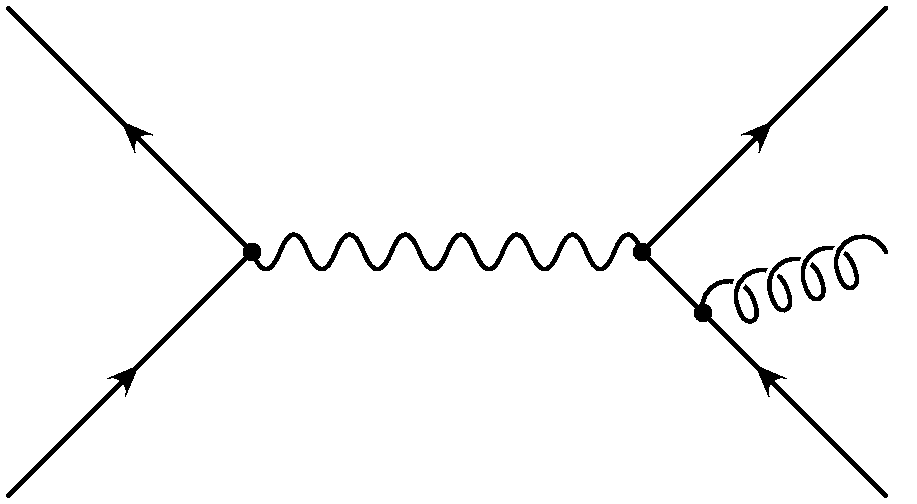
\includegraphics[width=\textwidth]{images/e+e-_real1.pdf}
	\end{subfigure}
	\hspace{1cm}
	\begin{subfigure}[]{0.45\textwidth}
		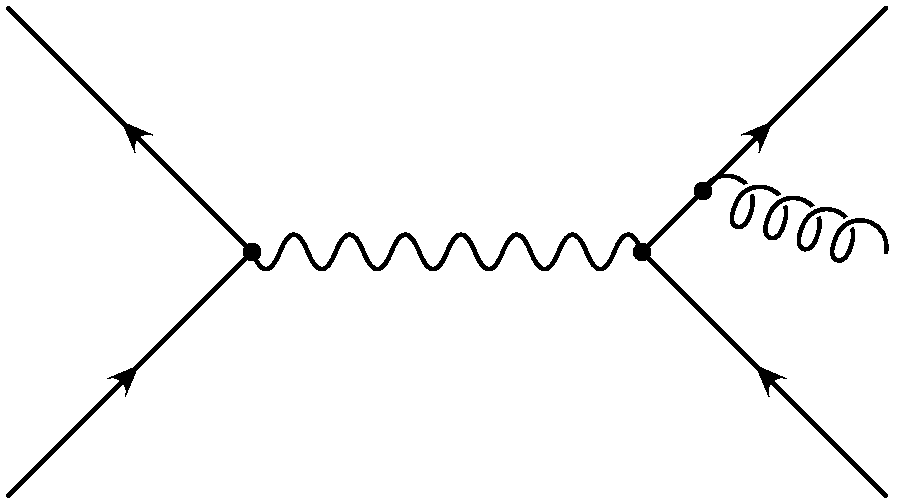
\includegraphics[width=\textwidth]{images/e+e-_real2.pdf}
	\end{subfigure}
	\caption{Feynman diagrams for gluon emission in $e^+ e^-$ annihilation}
	\label{fig:e+e-_real}
\end{figure}
%
Considering soft emission only, one can show that the differential cross section for this process factorizes so that one can write
%
\begin{equation}
  \abs{\matrixelement_{q \bar q g}}^2 \dif \Phi_{q \bar q g} \simeq \abs{\matrixelement_{q \bar q}}^2 \dif \Phi_{q \bar q} \dif \softgluon \, .
\end{equation}
%
The squared matrix element and phase space for $q \bar q$ production plus the emission of a soft gluon is given by the Born squared matrix element and phase space multiplied by a factor $\dif \softgluon$, which is the probability for the emission of a soft gluon:
%
\begin{equation}
  \dif \softgluon = \frac{2 \alpha_s C_F}{\pi} \frac{\dif E}{E} \frac{\dif \theta}{\sin \theta} \frac{\dif \phi}{2 \pi} \, .
\end{equation}
%
There are two divergences in this equation:
In the limit $E \rightarrow 0$ there is an infrared divergence and in the limit $\theta \rightarrow 0,\pi$ there is a collinear divergence when the gluon and quark move in the same direction.
These divergences always appear when a gluon is emitted by a quark \cite{salam2010}.

Additionally to the real emissions in \cref{fig:e+e-_real} there are virtual emissions shown in \cref{fig:e+e-_virtual}, which we have not taken into account yet.
%
\begin{figure}[]
	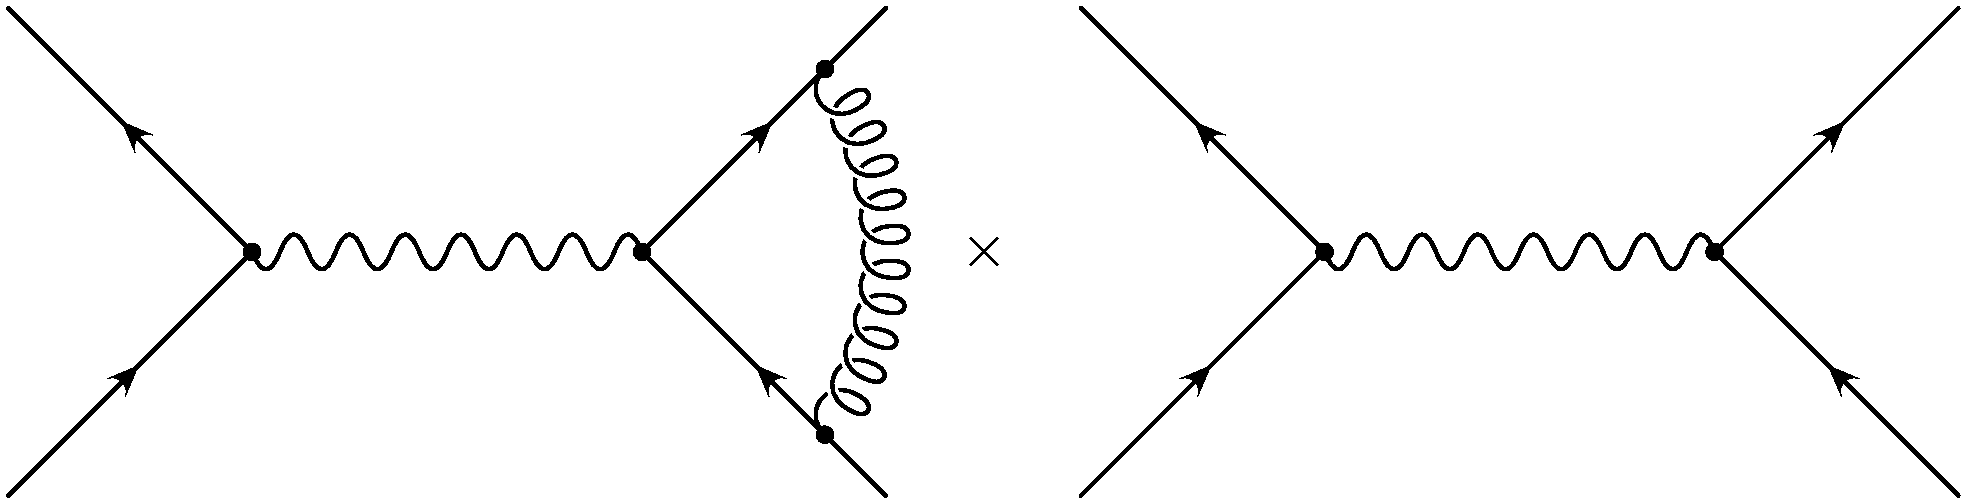
\includegraphics[width=\textwidth]{images/e+e-_virtual.pdf}
	\caption{Virtual correction in $e^+ e^-$ annihilation}
	\label{fig:e+e-_virtual}
\end{figure}
%
As the total cross section must be finite, the divergences in the real term must be canceled by the virtual term (this can, for example, be shown by the use of dimensional regularization \cite{ellis1996}).
Therefore the corrections to the total cross section are dominated by hard, large-angle gluons and for these perturbation theory is applicable \cite{salam2010}.
Observables that are insensitive to the emission of soft or collinear gluons, like the total cross section for $e^+ e^- \rightarrow \text{hadrons}$, are called \textit{infrared safe}.
%
\subsection{Factorization}
In processes involving initial-state hadrons, the partons can emit gluons before entering the hard interaction (see \cref{fig:initial_gluon}).
%
\begin{figure}
\centering
	\begin{subfigure}[]{0.3\textwidth}
		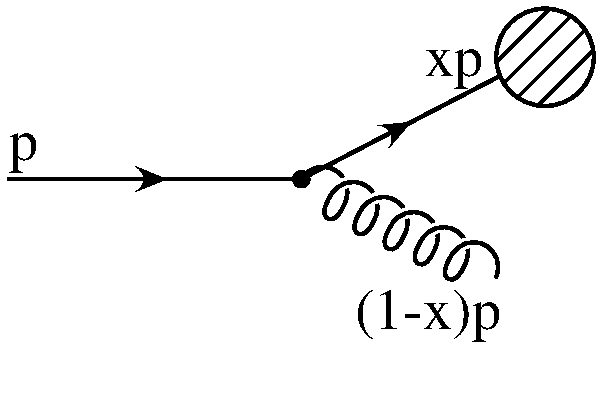
\includegraphics[width=\textwidth]{images/initial_real.pdf}
	\end{subfigure}
	\hspace{1cm}
	\begin{subfigure}[]{0.3\textwidth}
		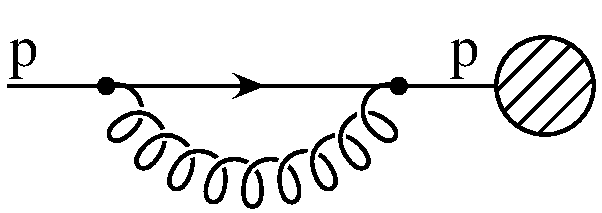
\includegraphics[width=\textwidth]{images/initial_virtual.pdf}
	\end{subfigure}
	\caption{Feynman diagrams for initial-state gluon emission}
	\label{fig:initial_gluon}
\end{figure}
%
However, there is an important difference between real and virtual emissions in this case:
While the virtual emission does not change the momentum of the parton entering the process, the real gluon carries off parts of the parton momentum.
Thus, the total cross section consists of two different hard cross sections that do not cancel in the collinear limit.
This is a consequence of the collinear limit corresponding to long-range effects of the strong interaction, which are not calculable in perturbation theory.

In order to be able to calculate cross sections with initial-state hadrons, we can take a similar approach as for the renormalization of the coupling constant and introduce a scale variable which we call the \textit{factorization scale} $\mu_F$.
All the non-perturbative parts are cut off at $\mu_F$ and absorbed into the PDF.
There is an arbitrariness in how much of the correction terms is to be factored out.
This is defined by the \textit{factorization scheme}.
Common schemes include the DIS scheme, in which all non-leading order contributions are absorbed into the PDFs, and the $\overline{MS}$ scheme, in which only the divergent parts are absorbed.
Once the factorization scheme has been chosen, it has to be used consistently in all following cross section calculations.
%
\subsection{Evolution}
There is an analog for the renormalization group equation for factorization, called the Dokshitzer-Gribov-Lipatov-Altarelli-Parisi (DGLAP) equation.
For a quark entering the hard process with longitudinal momentum $xp$ it takes the form
%
\begin{equation}
	\dod{q(x,\mu_F^2)}{\ln{\mu_F^2}} = \frac{\alpha_s}{2 \pi} \int_x^1 \dif z P_{qq}(z) \frac{q(x/z,\mu_F^2)}{z} \, ,
\end{equation}
%
where $q(x/z,\mu_F^2)$ is the quark distribution.
The function $P_{qq}(z)$ is called splitting kernel.
It has a perturbative expansion in $\alpha_s$:
%
\begin{equation}
	P_{qq}(z) = P_{qq}^{(0)}(z) + \frac{\alpha_s}{2 \pi} P_{qq}^{(1)}(z) + \dots \, .
\end{equation}
%
As the proton does not only contain quarks but also antiquarks and gluons, the actual DGLAP equation is a matrix equation:
%
\begin{equation}
	\dod{}{\ln{\mu_F^2}} \begin{pmatrix} q_i \\ g \end{pmatrix} = \frac{\alpha_s(\mu_F^2)}{2 \pi}
	\begin{pmatrix}
		P_{q_i q_j}	&	P_{q_i g} \\
		P_{g q_j}	&	P_{gg}
	\end{pmatrix}
	\otimes \begin{pmatrix} q_j \\ g \end{pmatrix} \, .
	\label{eq:dglap}
\end{equation}
%
All splitting kernels can be written as perturbative series and have been calculated up to next-to-next-to-leading-order\cite{splittingkernel1,splittingkernel2}. 
The DGLAP equation allows to calculate the scale dependence of the PDFs and therefore is an important and powerful tool for PDF fits.
%
\section{Parton shower}
There are phase space regions that cannot be well described by fixed order calculations in perturbation theory.
These include collinear parton splitting and soft gluon emission, which are closely related to the presence of infrared divergences.
To describe them accurately, higher order terms need to be considered.
However, the work required to derive the needed matrix elements quickly increases with each order, which is the reason why most processes have not been calculated further than NLO.
We need a different approach to deal with the problematic phase space regions.
Instead of relying on a fixed order calculation, we can consider an approximate model that includes the dominant contributions at all orders.
In this model, the collinear splitting and soft gluon emission of every parton in the initial and final state is simulated with respect to the related probabilities.
The additional partons are again able to split or radiate gluons.
By recursively applying this procedure, we obtain a cascade of parton emissions, called a \textit{parton shower}.
An example is illustrated in \cref{fig:partonshower}.
The shower ends when a certain cut-off scale is reached.
%
\begin{figure}[]
	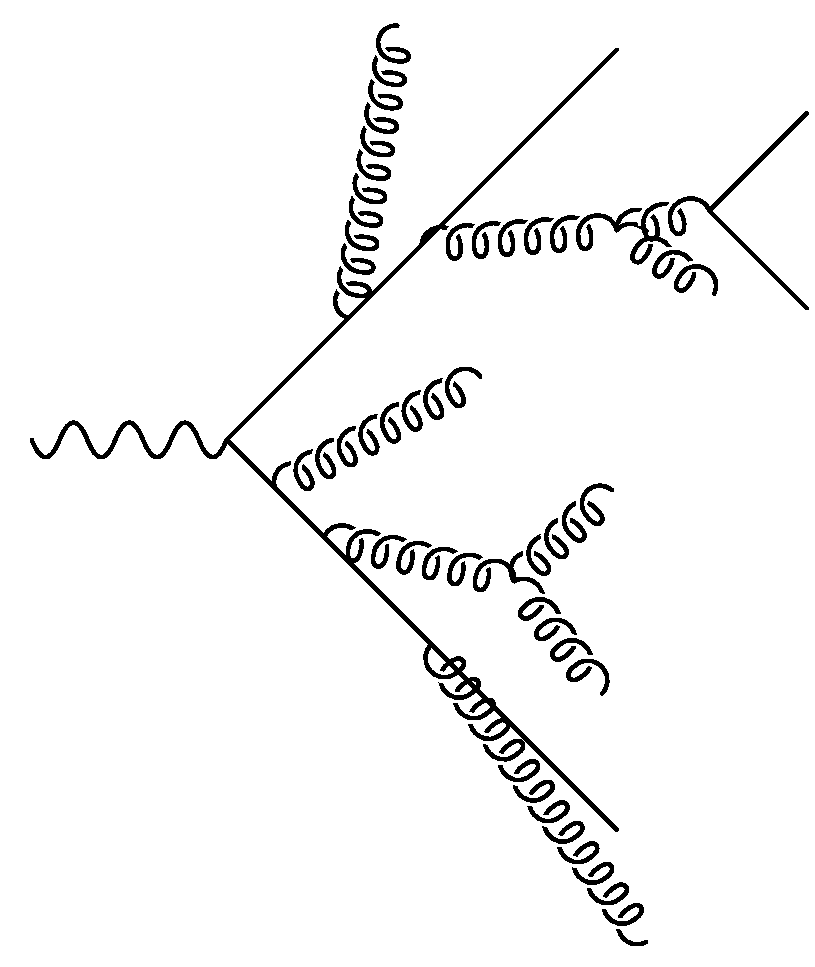
\includegraphics[width=0.5\textwidth]{images/partonshower.pdf}
	\caption{Example of a parton shower.}
	\label{fig:partonshower}
\end{figure}
%

The evolution of the splitting with the decreasing scale is given by the DGLAP equation \cref{eq:dglap}.
In this context the PDFs do not describe the momentum distributions of the partons inside of a hadron, but rather the distribution of the momentum fractions of the partons resulting from the splitting.

The computation of parton showers can be formulated in a way that is well suited for a Monte Carlo program.
We can combine the parton shower program with a hadronization model, that combines both the initial state and the final state partons into colorless hadrons, beginning at the cutoff scale of the shower. We call the result a \textit{parton shower Monte Carlo event generator}.
It is a powerful tool that is able to fully simulate QCD events in hadron collisions.

The main disadvantage of parton shower generators is that they are not guaranteed to properly describe events that include hard and large-angle emissions.
Those events are, however, correctly described by fixed order calculations.
To combine the benefits of both, algorithms have been developed that merge LO matrix elements and parton showers with different multiplicities (MEPS).
The main issue in the course of this is double counting.
An event with $n$ partons in the final state can either be the product of an $n$-parton matrix element that has been showered with only soft and collinear emissions or it could be the product of an $(n-1)$-parton matrix element for which the showering led to the emission of a hard, large-angle gluon.
Those cases have to be carefully seperated to avoid an overrepresentation of the related phase space region.
The most widely used methods to avoid double counting are CKKW matching \cite{ckkw_a,ckkw_b} and MLM matching \cite{mlm_a,mlm_b}.

Another problem of parton shower predictions is that they suffer from strong scale dependence because they are based on LO matrix elements.
Promoting parton showers to NLO accuracy is a much harder task because of divergent event weights.
Nonetheless, there are methods to circumvent this problem and the two widely used solutions are \mcatnlo{} \cite{mcatnlo} and \powheg{} \cite{powheg_a,powheg_b,powheg_c}.
As of recently, it is also possible to merge different jet multiplicities in NLO calculations matched to parton showers \cite{nlomerging1,nlomerging2,nlomerging3,nlomerging4,nlomerging5}.
%
\section{Next-to-leading order calculations}
\label{sec:nlo_calculations}
\ldots(need real and virtual, both seperately divergent, need to regularize)


There are two general methods that are commonly used to take care of the infrared divergences in NLO calculations, namely the \textit{slicing method} and the \textit{subtraction method}.
The slicing method introduces a small parameter $\delta$, which slices the integration region into two pieces so that it can be computed numerically.
A residual dependency on $\delta$ remains, which should be neglectable if $\delta$ is small.
However, this has to be checked in an actual calculation.
The advantage of the subtraction method is that it does not involve any approximations.

We can demonstrate the subtraction method with a simple example, that has been adopted from \cite{mcatnlo}.
Consider the expression for the expectation value of an infrared-safe observable $O$ at NLO accuracy, consisting of a Born (B), a virtual (V) und a real (R) term:
%
\begin{equation}
	\left< O \right> = \lim_{\epsilon \rightarrow 0} \int_0^1 \dif x x^{-2 \epsilon} O(x) \left[ \left( \od{\sigma}{x} \right)_B + \left( \od{\sigma}{x} \right)_V + \left( \od{\sigma}{x} \right)_R \right] \, .
\end{equation}
%
We assume that the cross sections can be written as
%
\begin{align}
	\left( \od{\sigma}{x} \right)_B &= B \delta(x) \, , \\
	\left( \od{\sigma}{x} \right)_V &= a \left( \frac{B}{2 \epsilon} + V \right) \delta(x) \, , \\
	\left( \od{\sigma}{x} \right)_R &= a \frac{R(x)}{x} \,
\end{align}
%
where $B$ and $V$ are constant factors and $\lim_{x \rightarrow 0} R(x) = B$.
$a$ denotes the coupling constant.
Obviously, both the real and the virtual part are divergent in the limit $\epsilon \rightarrow 0$.
Using the subtraction method, we can rewrite the real contribution to obtain
%
\begin{align}
	\left< O \right>_R	&= a \lim_{\epsilon \rightarrow 0} \int_0^1 \frac{\dif x}{x^{1+2 \epsilon}} O(x) R(x) \nonumber \\
						&= a B O(0) \lim_{\epsilon \rightarrow 0} \int_0^1 \frac{\dif x}{x^{1+2 \epsilon}} + a \int_0^1 \frac{\dif x}{x} [O(x) R(x) - B O(0)] \nonumber \\
						&= -a B O(0) \lim_{\epsilon \rightarrow 0} \frac{1}{2 \epsilon} + a \int_0^1 \frac{\dif x}{x} [O(x) R(x) - B O(0)] \, .
	\label{eq:toymodel_realsub}
\end{align}
%
By explicitely writing down the virtual part,
%
\begin{equation}
	\left< o \right>_V = a \lim_{\epsilon \rightarrow 0} \int_0^1 \frac{\dif x}{x^{2 \epsilon}} O(x) \left( \frac{B}{2 \epsilon} + V \right) \delta(x) \, ,
\end{equation}
%
we see that the first term gets exactly cancelled by the first term on the right hand side of \eqref{eq:toymodel_realsub}.
Including the Born contribtion we arrive at the expression
%
\begin{equation}
	\left< O \right> = B O(0) + a \left\{ V O(0) + \int_0^1 \frac{\dif x}{x} [O(x) R(x) - B O(0)] \right\} \, ,
\end{equation}
%
which now only consists of finite terms.
The remaining integral can be evaluated using Monte Carlo methods.
The subtraction method can be generalized to arbitrary hadronic cross sections, provided that the definition of the observables allows the cancellation of the divergences.
%
\section{Reweighting QCD calculations}
Often it is needed to vary the parameters in QCD calculations, for example the scale variables and PDFs to estimate the uncertainty.
When the number of variations becomes large, it is not practical to rerun the whole event generation for each calculation as the time and resource consumption become too high.
Instead it is possible to reuse information from previously generated events and combine them with the new parameters.
Here we consider an NLO calculation using Catani-Seymour subtraction \cite{catani_seymour1997}, which is the scheme implemented in \sherpa{} and \mcgrid{}.
Other subtraction schemes can be used as well, as is demonstrated in \cite{amcfast} for the FKS scheme \cite{fks_a,fks_b}.

The total cross section can be separated into four finite terms:
%
\begin{equation}
	\sigma^\text{NLO}_{pp \rightarrow X} = \int \dif \hat \sigma^B + \int \dif \hat \sigma^V + \int \dif \hat \sigma^I + \int \dif \hat \sigma^{RS} \,
\end{equation}
%
They correspond to the Born (B), virtual (V), integrated subtraction (I) and real subtraction (RS) parts of the calculation.
We need to work out the explicit dependence on the parameters to accurately reweight them.

For the B and RS terms this is straightforward as they resemble LO calculations.
Making use of the factorization theorem we can write them in the form
%
\begin{equation}
	\sigma^{B/RS} = \sum_{i,j} \int \dif x_1 \dif x_2 \int \dif \Phi_n \left( \frac{\alpha_s(\mu_R^2)}{2 \pi} \right)^p \pdf_i(x_1,\mu_F^2) \pdf_j(x_2,\mu_F^2) \dif \hat\sigma \, ,
\end{equation}
%
where for the B term $p = p_\text{LO}$ and for the RS term $p = p_\text{LO} + 1$.
Using Monte Carlo integration, we can rewrite this as a sum over generated events:
%
\begin{equation}
  \int \dif \hat \sigma^{B/RS} = \sum_{e=1}^{N_\text{evt}} \alpha_s^p(\mu_R^2) \pdf_1(x_1,\mu_F^2) \pdf_2(x_2,\mu_F^2) w_e^{(0)} \, ,
  \label{eq:reweight_lo}
\end{equation}
%
where the weight $w_e^{(0)}$ contains the parton-level matrix element squared and is completely independent of the QCD input parameters.

The virtual part occupies a more complicated structure because the weights depend on the renormalization scale.
It takes the form
%
\begin{equation}
	\int \dif \hat \sigma^V = \sum_{e=1}^{N_\text{evt}} \alpha_s^{p_\text{LO} + 1}(\mu_R^2) \pdf_1(x_1,\mu_F^2) \pdf_2(x_2,\mu_F^2) \left\{ w_e^{(0)} + l_R w_e^{(1)} + l_R^2 w_e^{(2)} \right\} \, ,
\end{equation}
%
with renormalization scale logarithms $l_R = \log\left(\frac{\mu_r^2}{\mu_{R,0}^2} \right)$, where $\mu_{R,0}$ is the scale at which $w_e^{(1)}$ and $w_e^{(2)}$ were originally evaluated.

In the I part, the event weights have a complex dependence on the PDF.
The full structure can be written as
%
\begin{align}
	\int \dif \hat \sigma^I = \sum_{e=1}^{N_\text{evt}} &\alpha_s^{p_\text{LO} + 1}(\mu_R^2) \left\{ \vphantom{\left( \sum_{k=1}^4 \right)} f_1(i,x_1,\mu_F^2) w_e^{(0)} f_2(j,x_2,\mu_F^2) \right. \nonumber \\
								&+ \left( \sum_{k=1}^4 f_1^{(k)}(i,x_1,x'_1,\mu_F^2) w_{e,k}^{(3)} \right) f_2(j,x_2,\mu_F^2) \nonumber \\
								&\left. + f_1(j,x_1,\mu_F^2) \left( \sum_{k=1}^4 w_{e,k}^{(4)} f_2^{(k)}(j,x_2,x'_2,\mu_F^2) \right) \right\} \, ,
\end{align}
%
where the $x$ and $x'$ are the Björken-$x$ before and after initial state branching.
Moreover, $i$ and $j$ denote the parton flavours before the branching and the $f^{(k)}$ provide the correct form of the PDF depending on the type of branching.
They are given explicitly in \cite{mcgrid2013}.

We can dispose of the weights $w^{(1)}$ and $w^{(2)}$ by chosing a central scale.
If we furthermore project the contributions from $w^{(3)}$ and $w^{(4)}$ onto separate events, we can write the total NLO cross section in the compact form
%
\begin{equation}
  \sigma^\text{NLO}_{pp \rightarrow X} = \sum_{e=1}^{N_\text{evt}} \alpha_s^{p_e}(\mu_R^2) \pdf_1(x_1,\mu_F^2) \pdf_2(x_2,\mu_F^2) w_e \, ,
  \label{eq:reweight_nlo}
\end{equation}
%

Provided that all event weights have been stored, it is now possible to change the values of $\alpha_s$, $\mu_R$ and $\mu_F$ or use a different PDF \textit{a posteriori}.
%
\section{Interpolation grids}
Despite the advantage towards regenerating all events for the variation of a single parameter, the reweighting approach is still not a satisfying solution for many use cases.
The whole event record has to be stored, which can easily reach many gigabytes in high statistics computations.
The storing and reprocessing of the events may be a challenge by itself and is not convenient if more than a few parameter variations have to be performed.
One therefore whishes to somehow decrease the resource requirements without losing a significant amount of accuracy.
In the ideal case, it should be mostly independent on the statistics.
A possible solution is the use of interpolating grids to represent the PDFs and event weights.
Then only a uniquely defined number of values has to be saved, while values in-between the grid points are generated by interpolating functions.
Such a method has been implemented by the \appl{} \cite{applgrid2010} and \fnlo{} \cite{fastnlo2006,fastnlo2011} projects.

The PDF $\pdf(x,Q^2)$ depends on the momentum fraction $x$ and the momentum transfer $Q^2$.
It can be approximated as a sum over discrete grid points using interpolation functions $I$ of order $N$:
%
\begin{equation}
	\pdf(x,Q^2) = \sum_{i=0}^{N_x} \sum_{j=0}^{N_Q} \pdf(x_i,Q_j^2) I_i^{(N_x)}(x_1) I_j^{(N_Q)}(Q^2) \, .
\end{equation}
%
Consequently, we can write \cref{eq:reweight_nlo} as
%
\begin{alignat}{3}
  \sigma^\text{NLO}_{pp \rightarrow X}	&= \sum_{e=1}^{N_\text{evt}} \sum_{i,j=0}^{N_x} \sum_{k=0}^{N_Q} &&\alpha_s^{p_e}(Q_k^2) \pdf_1(x_i,Q_k^2) \pdf_2(x_j,Q_k^2) w_e \nonumber \\
  										&	&&\cdot I_i^{(N_x)}(x_1) I_j^{(N_x)}(x_2) I_k^{(N_Q)}(Q^2) \nonumber \\
  										&= \mathrlap{\sum_p \sum_{i,j=0}^{N_x} \sum_{k=0}^{N_Q} \alpha_s^p(Q_k^2) \pdf_1(x_i,Q_k^2) \pdf_2(x_j,Q_k^2) W_{i,j,k}^{(p)} \, ,}
\end{alignat}
%
where $p$ is the perturbative order and the interpolated weights $W_{i,j,k}^{(p)}$ are processed as a sum over the events:
\begin{equation}
	W_{i,j,k}^{(p)} = \sum_{e=1}^{N_\text{evt}} \delta_{p,p_e} w_e I_i^{(N_x)}(x_1) I_j^{(N_x)}(x_2) I_k^{(N_Q)}(Q^2) \, .
\end{equation}
%
Now the sum over the events has been completely absorbed into the definition of the interpolated weights.
These can be calculated in a single run of the event generator and be stored efficiently.
The calculation of the cross section has become a simple sum over the grid points and thus is much faster for a large number of events.
The approach can easily be extended to histogrammed data like differential cross sections by defining the observable bins and computing one weight $W_{i,j,k}^{(p),(s),(b)}$ for each bin $b$.
However, unlike the full event record, the weight grid is restricted to the observable it was constructed for and cannot be used to calculate any other values.

While the variation of the PDF and $\alpha_s$ is still straightforward, scale variation is slightly more complicated because the weights themselves depend on the scale choices.
Nevertheless, it is possible to vary the scales without too much effort, using DGLAP evolution.
The precise procedure is explained in \cite{applgrid2010}.
%
\section{The considered process: Higgs production through gluon fusion}
The Englert-Brout-Higgs-Guralnik-Hagen-Kibble mechanism (commonly Higgs mechanism) explains the non-zero masses of the gauge bosons in the standard model.
It has been developed in the 1960s with important contributions coming from several people \cite{higgs1964a,higgs1964b,englert1964,guralnik1964,nambu1960,anderson1963}.
It invokes the process of spontaneous symmetry breaking and evades the Goldstone theorem.
In the development of the standard model, the Higgs mechanism played a key role and ever since the discovery of the Higgs boson in 2012 by ATLAS \cite{higgsdiscovery_atlas2012} and CMS \cite{higgsdiscovery_cms2012} at the LHC it has received wide approval.

In this thesis, the considered process will be the production of a Higgs boson through gluon fusion.
Although there are other possible production mechanisms in the Standard Model, this is the main process at the LHC, with an expected cross section of $\approx \SI{50}{\pico\barn}$ at a center-of-mass energy of $\sqrt{s} = \SI{14}{\tera\electronvolt}$ and a Higgs mass of $\SI{125}{\giga\electronvolt}$ \cite{higgshandbook1}.
It proceeds through a triangular loop of heavy quarks (mainly top quarks as the Higgs coupling scales with the quark mass) as is shown in \figref{fig:gluonfusion}.
%
\begin{figure}[]
	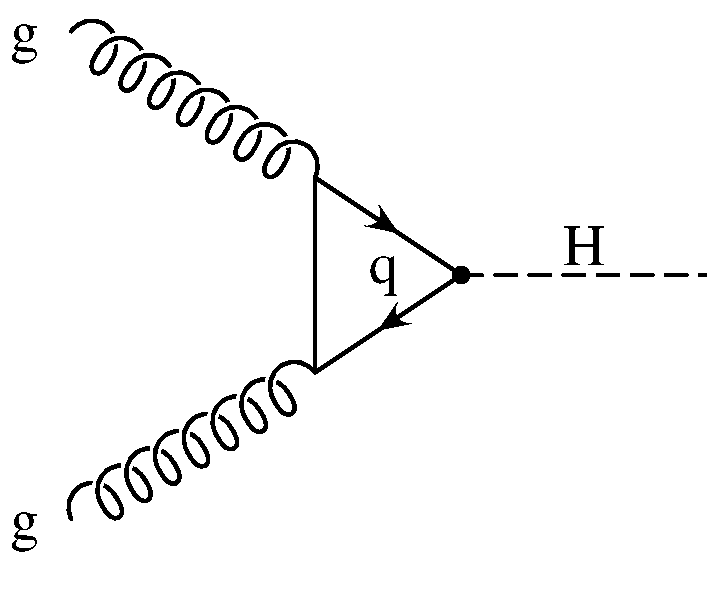
\includegraphics[width=0.5\textwidth]{images/gluonfusion.pdf}
	\caption{Higgs production through gluon fusion.}
	\label{fig:gluonfusion}
\end{figure}
%

In the narrow-width approximation, the leading order cross section is given by \cite{gluonfusioncrosssection}
%
\begin{equation}
	\sigma_\text{LO}(pp \rightarrow H) = \sigma_0^H \tau_H \od{\lumi^{gg}}{\tau_H} \, ,
\end{equation}
%
where $\tau_H = M_H^2/s$ is the Drell-Yan variable and $\dif \lumi^{gg} / \dif \tau_H$ is the gluon luminosity.
The partonic cross section $\sigma_0^H$ can be written as
\begin{equation}
	\sigma_0^H = \frac{G_F \alpha_s^2(\mu_R^2)}{288 \sqrt{2} \pi} \abs{ \sum_q \frac{3}{2 \tau_q} \left[ 1 + \left( 1 - \frac{1}{\tau_q} \right) f(\tau_q) \right] }^2  \, ,
\end{equation}
%
with the form factor
%
\begin{equation}
	f(\tau_q) = 
	\begin{cases}
		\arcsin^2 \left( \sqrt{\tau_q} \right) ,																& \tau_q < 1, \\
		- \frac{1}{4} \left[ \ln \frac{1 + \sqrt{1-\tau_q^{-1}}}{1 - \sqrt{1-\tau_q^{-1}}} -i \pi \right]^2 ,	& \tau_q > 1,
	\end{cases}
\end{equation}
%
where $G_F$ denotes the Fermi coupling constant and $\tau_q = m_H^2/4m_q^2$.
The gluon luminosity takes the form
%
\begin{equation}
	\od{\lumi^{gg}}{\tau_H} = \int_0^1 \dif x_1 \dif x_2 \gluonpdf(x_1,\mu_F^2) \gluonpdf(x_2,\mu_F^2) \delta(x_1 x_2 - \tau_q) \,
\end{equation}
%
with $\gluonpdf(x,\mu_F^2)$ denoting the gluon PDF.

The QCD corrections are composed of virtual corrections to the vertices and propagators, real gluon radiation in the initial state and the contributions of the subprocesses $gq \rightarrow Hq$ and $q \bar q \rightarrow Hg$.
Exemplary diagrams for the corrections are shown in \figref{fig:ggh_corrections}.
The full NLO cross section has been calculated in \cite{gfusionnlo1,gfusionnlo2,gfusionnlo3}.
They increase the cross section by a factor of \num{1.5} to \num{1.7}.
%
\begin{figure}
\centering
\begin{subfigure}[]{0.3\textwidth}
	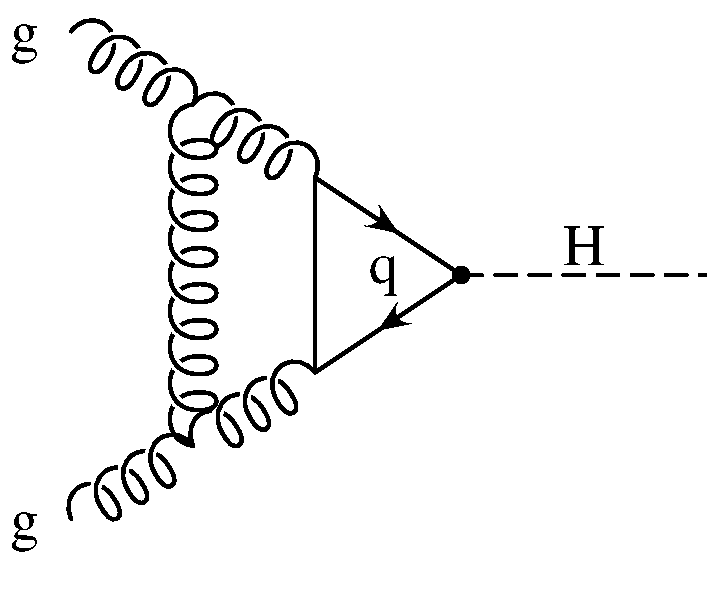
\includegraphics[width=\textwidth]{images/gluonfusion_virtual1.pdf}
	\caption{}
\end{subfigure}
~
\begin{subfigure}[]{0.3\textwidth}
	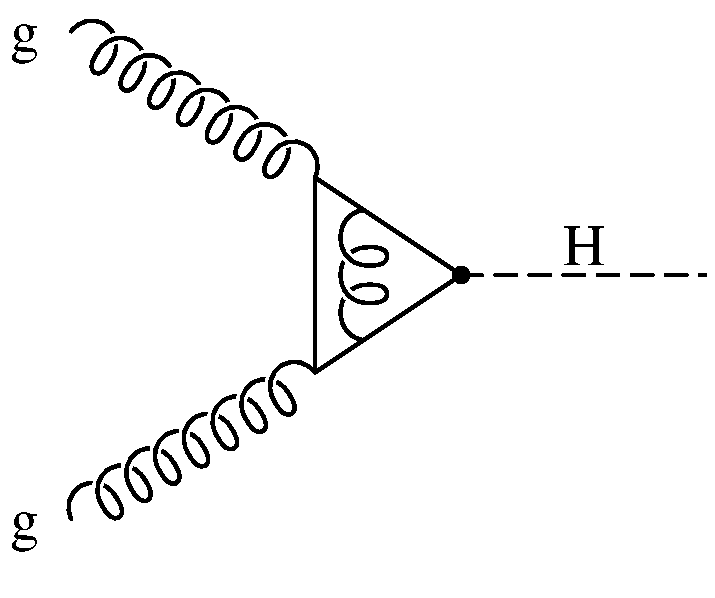
\includegraphics[width=\textwidth]{images/gluonfusion_virtual2.pdf}
	\caption{}
\end{subfigure}
~
\begin{subfigure}[]{0.3\textwidth}
	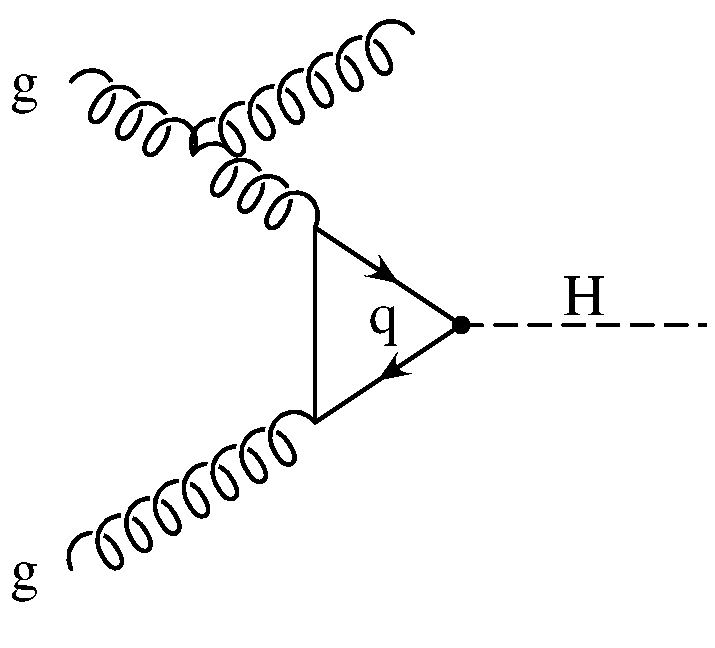
\includegraphics[width=\textwidth]{images/gluonfusion_real1.pdf}
	\caption{}
\end{subfigure}

\begin{subfigure}[]{0.3\textwidth}
	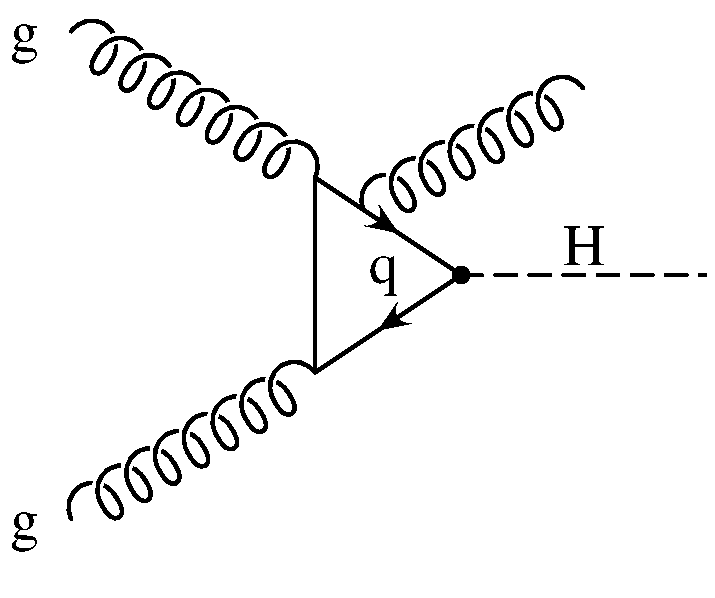
\includegraphics[width=\textwidth]{images/gluonfusion_real2.pdf}
	\caption{}
\end{subfigure}
~
\begin{subfigure}[]{0.3\textwidth}
	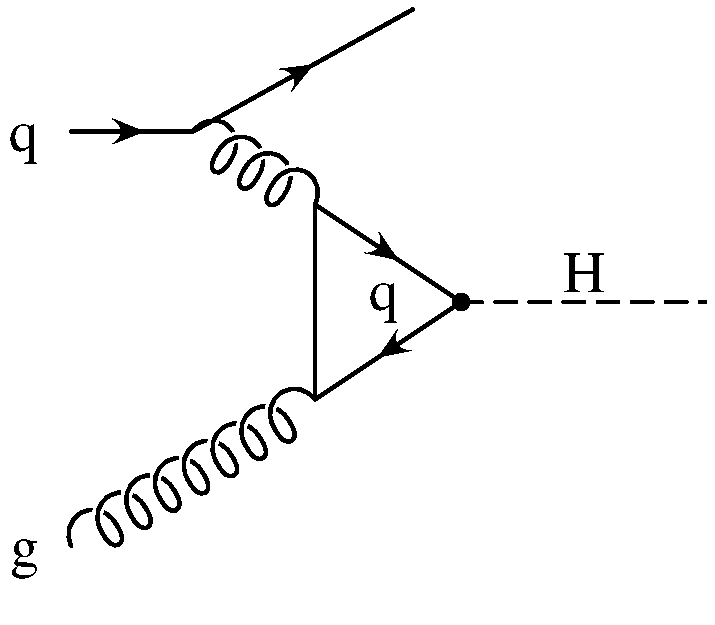
\includegraphics[width=\textwidth]{images/gq_hq.pdf}
	\caption{}
\end{subfigure}
~
\begin{subfigure}[]{0.3\textwidth}
	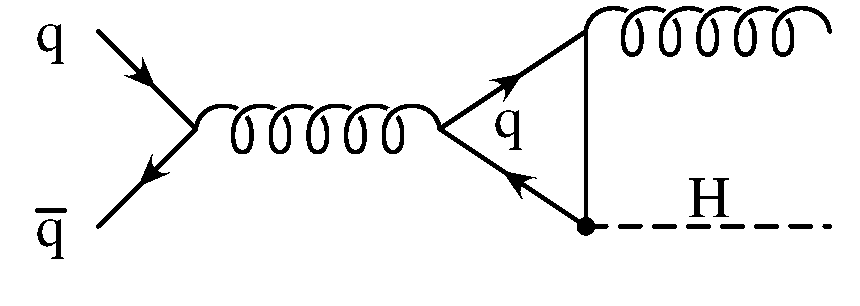
\includegraphics[width=\textwidth]{images/qq_hg.pdf}
	\caption{}
\end{subfigure}
\caption{Example diagrams illustrating the QCD corrections to the process $pp \rightarrow H$:
		(a), (b) virtual corrections; (c), (d) real emission of a gluon; (e) $gq \rightarrow Hq$; (f) $q \bar q \rightarrow Hg$.}
\label{fig:ggh_corrections}
\end{figure}
%

In the limit where the top quark has infinite mass, $m_t \rightarrow \infty$, the form factor takes the value $\frac{4}{3}$.
This allows for an analytical expression of the corrections \cite{gfusionnlo2}.
It can be considered as an extension of the Standard Model, where the Higgs boson couples directly to gluons, known as effective Higgs coupling (cf. \cref{fig:heft}).
The effective Lagrangian for Higgs gluon interaction can be written as \cite{gfusionnnlo2}
%
\begin{equation}
	\Lagr_\text{eff}^{ggH} = - \frac{1}{4v} C_1 G_{\mu \nu}^a {G^a}^{\mu \nu} H \, ,
\end{equation}
%
where $v$ is the Higgs vacuum expectation value, $G^a_{\mu \nu}$ is the gluon field strength tensor and $H$ is the Higgs field.
The coefficient $C_1$, in the \msbar{} scheme, is given by
%
\begin{align}
	C_1 = \frac{-1}{3 \pi} &\left\{1 + \frac{11 \alpha_s}{4 \pi} + \left( \frac{\alpha_s}{\pi} \right)^2 \left[ \frac{2777}{288} + \frac{19}{16} \log\left( \frac{\mu^2}{m_t^2} \right)
	\vphantom{n_f \left( -\frac{67}{96} + \frac{1}{3} \log\left( \frac{\mu^2}{m_t^2} \right) \right)} \right. \right. \nonumber \\
	%	
		&\qquad \left. \left. \vphantom{\frac{2777}{288} + \frac{19}{16} \log\left( \frac{\mu^2}{m_t^2} \right)}
		+ n_f \left( -\frac{67}{96} + \frac{1}{3} \log\left( \frac{\mu^2}{m_t^2} \right) \right) \right] + \order{\alpha_s^3} \right\} \, ,
\end{align}
%
where the number of active flavors should be set to $n_f = 5$.
According to \cite{gfusionnnlo2}, at LO this approximation is accurate within \SI{5}{\percent} for $m_H \approx \SI{150}{\giga\electronvolt}$ (which is close to the measured value $m_H \approx \SI{126}{\giga\electronvolt}$) and improves at NLO.
All calculations in this thesis are based on effective Higgs coupling.
%
\begin{figure}[]
	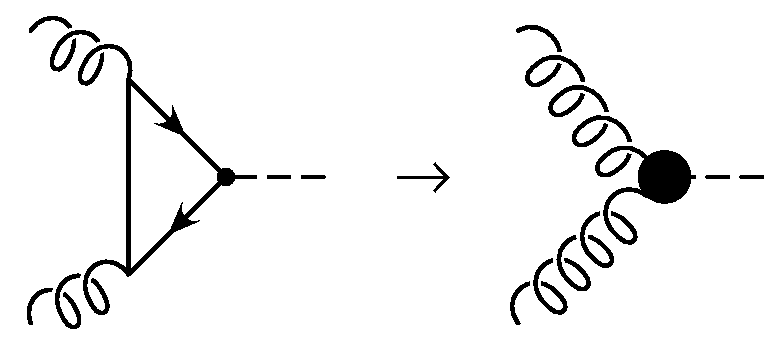
\includegraphics[width=0.5\textwidth]{images/heft.pdf}
	\caption{Effective Higgs coupling.}
	\label{fig:heft}
\end{figure}
%

Besides the basic process, the fully differential NLO cross sections are available for $H + 1$ jet \cite{gghj_nlo_fullydiff_1,gghj_nlo_fullydiff_2}, $H + 2$ jets \cite{gghjj_nlo_fullydiff_1,gghjj_nlo_fullydiff_2} and $H + 3$ jets \cite{gghjjj_nlo_fullydiff}.
A fully differential NNLO calculation exists for $H + 0$ jets production \cite{ggh_nnlo_fullydiff_1,ggh_nnlo_fullydiff_2} and substantial progress has been achieved towards an NNLO calculation of the $H + 1$ jets cross section \cite{gghj_nnlo_progress}.
%
\section{Leptonic Higgs decay}
In an experiment, one would never observe the Higgs boson directly but rather reconstruct it from the measured properties of its decay products.
We want to approximate this situation by simulating the Higgs boson decay.
There are several possible decay channels.
One has to keep in mind that the Higgs coupling is proportional to the particle masses, so that it will decay into the heaviest possible particles.
Assuming a Higgs mass of $m_H = \SI{126}{\giga\electronvolt}$, the most relevant decay products are $q \bar q$ (where q denotes a bottom or charm quark), $WW$, $ZZ$, $Z \gamma$, $\gamma \gamma$, $gg$ and $\tau^+ \tau^-$ \cite{higgshandbook2}.
The decay into photons or gluons is only possible through intermediate loops.
The studies leading to the discovery of the Higgs boson at the LHC relied primarily on the decay modes $H \rightarrow \gamma \gamma$, $H \rightarrow ZZ$ and $H \rightarrow WW$.

For the purpose of this thesis, we will consider the decay $H \rightarrow \tau^+ \tau^-$, which has a branching ratio of approximately \SI{6}{\percent} \cite{higgshandbook3}.
The Feynman diagram is shown in \cref{fig:h_tautau}.
It would be possible to simulate the other decay channels as well, however, this would only complicate the analysis unnecessarily.
The leptonic decay is the easiest one and closely resembles the Drell-Yan process.
There have been searches for $H \rightarrow \tau \tau$ events in the LHC data and both ATLAS \cite{htau_atlas} and CMS \cite{htau_cms} have published evidence for this type of decay.
It also allows for the observation of additional jets that are produced in the initial state and are separated from the Higgs decay products.
We will not consider the further decay of the tau leptons, which would naturally occur in the experiment.
%
\begin{figure}[]
	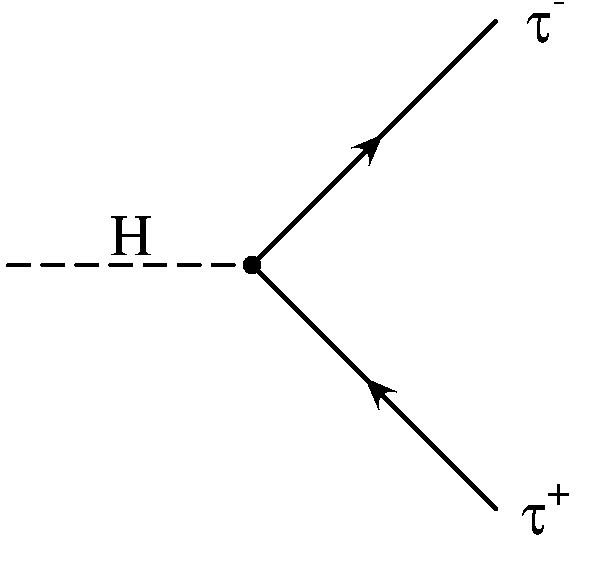
\includegraphics[width=0.5\textwidth]{images/h_tautau.pdf}
	\caption{Higgs decay into two $\tau$ leptons.}
	\label{fig:h_tautau}
\end{figure}
%
